\chapter{Risultati e sviluppi futuri}
\label{chap:risultati}

\section{Testing e analisi dei risultati}

\subsection{Modalità del testing}

Ai fini di testare la qualità del prodotto sviluppato, si è scelto di condurre una fase di testing verso la fine dei lavori, difatti, ad inizio progetto, sono state pianificate due sessioni di testing. Dopo qualche mese dall'inizio della tesi, sono stati inquadrati meglio i ruoli delle due sessioni: il primo round è stato concepito per testare le meccaniche base del gioco, e quindi capire se la demo diverte il giocatore, nonostante la grafica scarna di dettagli; mentre il secondo avrebbe avuto lo scopo di limare tutte le imperfezioni emerse dal primo test e quindi curare meglio la fruizione dei contenuti, cosa possibile dopo aver fissato per bene il gameplay di base.

Entrambi i test hanno avuto come giocatori dei ragazzini dall'età compresa fra i 12 e i 16 anni. Per il primo ci si è recati presso un oratorio Salesiano nel quartiere San Salvario di Torino verso la fine di Luglio 2015, qui l'età media dei giocatori è risultata essere fra i 12 e i 14 anni. Il secondo si è invece svolto ad inizio Ottobre 2015 presso l'istituto ITIS Majorana. Fra le due sessioni, è stato impiegato un mese per la revisione del design in base ai feedback ricevuti durante la prima sessione (vedremo nel dettaglio le scelte prese nella sezione \ref{revisione}).

In entrambe le sessioni, è stato seguito questo flow:

\begin{itemize}

\item Apertura: il referente interno introduce e-Mentor e i tesisti per spiegare cosa sta per succedere, quindi avviene una fase di presentazione dell'azienda e del progetto.
\item Preparazione al testing: a questo punto, si spiega qualche dettaglio sulle fasi dello sviluppo di un videogame (Pre-Production, Production etc), e si parla dell'attuale fase in cui ci si trova, cioè quella di testing, motivandone l'importanza, e il ruolo attivo che deve avere un tester.
\item Playtesting: senza fornire ulteriori dettagli sul gioco, i giocatori iniziano tutti a giocare contemporaneamente, dando loro istruzioni di comunicare e collaborare il meno possibile durante la partita.
\item Questionari: dopo 30-40 minuti (tempo ritenuto necessario per completare la demo fornita), viene fatto fermare il gioco a tutti i tester, ai quali è fornito un questionario da compilare (tramite scala di Likert).
\item Chiusura: a questo punto si spiega meglio cosa sia successo, e avviene una sessione di domande e risposte.
\item Raccolta dati: dopo aver finito la chiusura, si passa alla raccolta dati presenti sui computer dei tester, dati che verranno in seguito analizzati.

\end{itemize}

In entrambi i test, il pubblico si è mostrato molto entusiasta e collaborativo, favorendo il buon svolgimento della sessione. In totale, fra pre-testing, prima e seconda sessione di testing, il gioco è stato provato da oltre 70 persone.


\newpage

%--------------
%--------------

\subsection{Prima sessione di testing}

%--------------
%--------------
\subsubsection{Esito questionari}

La prima sessione di testing, come già detto, si è svolta presso un oratorio Salesiano verso fine Luglio 2015. Prima di effettuare questo testing, sono stati svolti vari test interni, i quali avevano come pubblico colleghi di e-Mentor e altri conoscenti vari, tutto ciò allo scopo di avere dei pareri super partes sul primissimo prototipo del gioco, il quale era stato visto soltanto dagli sviluppatori, fino a quel momento. 

Per motivi di logistica, dovuti alle attività organizzate dall'oratorio, sono state svolte tre mini sessioni di testing, facendo giocare 5-6 ragazzini alla volta.

I giocatori hanno mostrato grande spirito di partecipazione al gioco, e nonostante in alcuni tratti la difficoltà fosse alta, questi non sembravano essere stressati da ciò, continuando a riprovare.

\begin{figure}[h]
\centerline{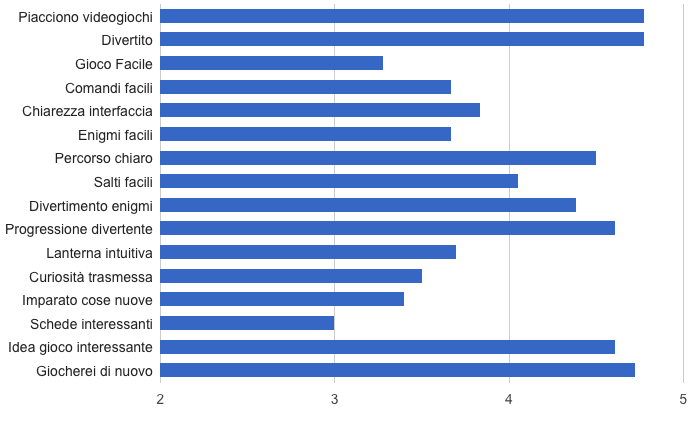
\includegraphics[scale=0.55]{images/risultati/test_01_questionario.png}}
\caption{Grafico sui questionari.}
\label{fig:test-questionario01}
\end{figure}

I questionari consistevano in domande e affermazioni, sulle quali il giocatore doveva esprimere il suo indice di gradimento tramite la scala Likert.
Vediamo ora, in base ai risultati mostrati in \myfig{\ref{fig:test-questionario01}}, ciò che si è evinto dai questionari forniti (dei quali è mostrata una media delle risposte):

\begin{itemize}

\item Piacciono i videogiochi: si è chiesto ad ogni giocatore se questo fosse abituato a giocare ai videogame, giusto per capire se fosse un videogiocatore abituale. Il voto medio finale è stato poco al di sotto di 5, quindi, quasi tutti i tester erano giocatori abituali.
\item Divertito: si è chiesto se il gioco abbia divertito in generale. La risposta media è stata molto alta, quasi pari a 5.
\item Facile: la domanda cerca di capire con quale difficoltà il gioco sia stato recepito. La media è stata poco superiore al 3, quindi il gioco è stato recepito come mediamente difficile.
\item Comandi Facili: la domanda mira a capire con quanta facilità sono stati usati i comandi di gioco. La media è stata poco al di sopra di 3,5.
\item Chiarezza interfaccia: si è cercato di capire se le varie interfacce di gioco, come quella in game o quella dei menù, fossero chiare. La risposta si è assestata poco sotto il 4.
\item Enigmi facili: anche qui si è cercato di capire la difficoltà avuta dai giocatori nel superare le parti puzzle del gioco. La votazione è stata poco superiore a 3,5, quindi gli enigmi sono stati mediamente difficili.
\item Percorso chiaro:  la domanda cerca di capire quanto chiaro e lineare fosse il gioco. La risposta è intorno al 4,5.
\item Salti facili: poiché nei test precedenti alla prima sessione, alcuni tester avevano avuto difficoltà nell'usare il salto durante il gioco, si è scelto di porre questa domanda. L'esito (media del 4 circa) ha confermato una minima, ma presente, difficoltà nell'usare i salti. 
\item Divertimento enigmi: i giocatori si sono divertiti abbastanza a risolvere gli enigmi, dando una valutazione media intorno al 4,5.
\item Progressione divertente: i giocatori, più andavano avanti e più si divertivano (sopra il 4,5).
\item Immediatezza lanterna: poiché la meccanica della Lanterna Magica è il fulcro del gioco, se ne è chiesta l'immediatezza. La risposta si è assestata verso il 3,7.
\item Curiosità trasmessa: poiché il gioco si propone di fornire informazioni e curiosità riguardo il pre-cinema, è stato chiesto al giocatore quanta curiosità questo gioco abbia fatto venire in lui riguardo l'ambito del pre-cinema. La risposta media è stata intorno a 3,5, quindi mediamente poco.
\item Imparato nuove cose: si è chiesto se il giocatore avesse appreso nuove nuove e la risposta è stata intorno a 3,4.
\item Schede interessanti: la risposta media è stata poco sopra il 3,5.
\item Idea gioco interessante: l'esito è stato molto positivo, assestandosi intorno a 4,5.
\item Giocherei di nuovo: anche qui, esito abbastanza positivo con valori intorno 4,7.

\end{itemize}

Nota bene: le domande fornite nei questionari sono state poste in modo più chiaro e verboso rispetto alle voci elencate precedentemente.

In base alle risposte discusse poco sopra, si è quindi evinto che il gioco è stato recepito molto bene dal pubblico, il quale si è divertito molto, ma il livello di difficoltà globale e l'immediatezza di tutorial ed interfacce di gioco, sono da rivedere. Inoltre, la fruizione dei contenuti informativi non è avvenuta nel migliore dei modi.
Si pensa inoltre, che la difficoltà avuta dai giocatori, nel muoversi all'interno del gioco, sia dovuta ai comandi a loro non particolarmente familiari, come la configurazione mouse e tastiera (che prevede l'uso dei tasti wasd).

%--------------

\subsubsection{Esito analisi oggettive}

Come spiegato nella sezione sulle modalità di testing, sono stati implementati ed usati degli strumenti ad hoc per analizzare oggettivamente il comportamento dei giocatori.
Queste analisi oggettive prevedono lo studio riguardo:

\begin{itemize}

\item tempo speso dall'utente per ogni sezione di gioco;
\item numero game over per zona;
\item collezionabili raccolti;
\item tempo dedicato alla lettura delle schede informative;

\end {itemize}

Vediamo quindi, i grafici, uno per livello, riguardo i tempi spesi dal giocatore per ogni sezione di gioco.

E' visibile in \myfig{\ref{fig:test_analisi_tempi_01}}  il grafico che mostra sulle ascisse le sezioni del livello e sulle ordinate il tempo speso (in secondi). Sono visibili 3 funzioni dal colore diverso:

\begin{itemize}

\item Medie reali (blu): sono i tempi mediati dei giocatori del test, quindi dei tempi reali;
\item Tempi ideali (*) (rosso): sono i tempi di gioco previsti per un giocatore esperto, cioè il tempo minimo che occorre spendere per quella sezione di gioco al fine di superare eventuali puzzle e raccogliere eventuali collezionabili;
\item Tempi previsti (**) (arancione): sono i tempi previsti, e diversamente da quelli ideali, tengono conto delle possibili difficoltà che un utente medio può avere, e quindi dei relativi tempi aggiuntivi.

\end {itemize}

Questo schema è stato usato anche per i prossimi livelli (e quindi i prossimi grafici), l'obiettivo di questa impostazione è capire quanto i grafici blu (tempi reali) si avvicinino a quelli arancioni (tempi previsti), più saranno simili, più il design realizzato avrà raggiunto il suo scopo. I tempi ideali servono invece a capire se un utente ha fatto qualcosa di strano in quella sezione, come per esempio non raccogliere un collezionabile e andare avanti nel gioco, oppure sfruttare un bug per risolvere la sezione prima del previsto, anzi, prima del tempo ideale, tempo minimo necessario per risolvere quella sezione.

Nota bene: Le sezioni aventi dei collezionabili secondari presentano un asterisco (*) nel nome. 

\begin{figure}[h]
\centerline{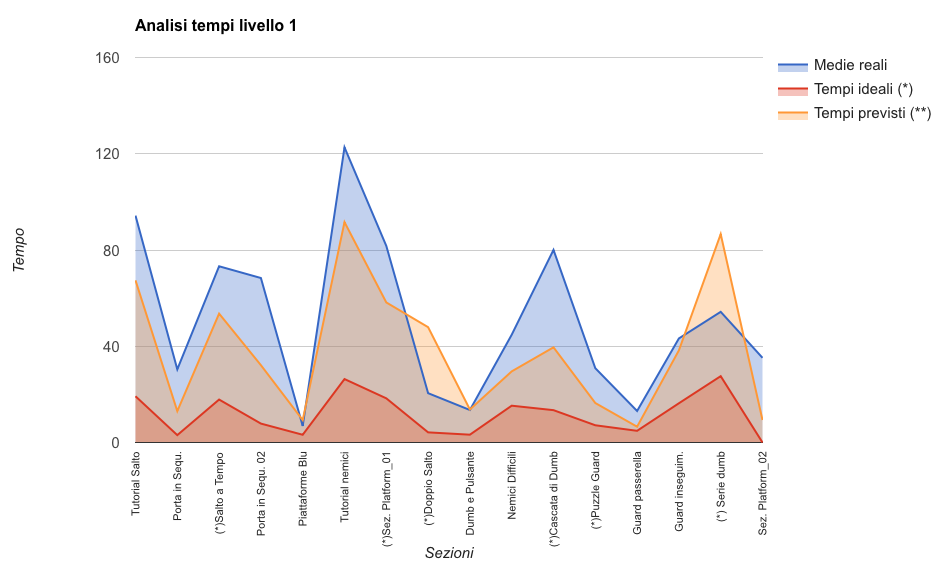
\includegraphics[scale=0.45]{images/risultati/test_01_analisi_tempi_01.png}}
\caption{Grafico analisi oggettiva dei tempi impiegati del livello 1.}
\label{fig:test_analisi_tempi_01}
\end{figure}

Il primo livello è risultato essere quello più ostico. Come si evince dal grafico, nelle sezioni ``Porta in sequ. 02'', ``Tutorial nemici'', ``Sez. platform 01'' e ``Cascata di dumb'', i tempi reali si sono discostati non poco da quelli previsti. Questa è la conferma oggettiva che il gioco ha presentato una difficoltà più alta di quella prevista, soprattutto riguardo le sezioni platform del gioco, non sempre ``comode'' da affrontare. Le sezioni di gioco proposte, probabilmente, richiedevano un'esperienza al giocatore troppo alta dopo solo qualche minuto di gameplay.

Il secondo livello, il cui grafico è mostrato in \myfig{\ref{fig:test_analisi_tempi_02}}, è stato recepito un po meglio rispetto al primo, tranne che in due sezioni: ``Tutorial Lanterna'' e ``Puzzle guard 01''. Mentre la seconda sezione ha un puzzle probabilmente troppo avanzato rispetto alla progressione di gioco, la prima, contiene il tutorial della Lanterna e quindi le prime verifiche sulla meccanica appena appresa. Questa sezione, come già detto durante l'analisi dei questionari, non è stata particolarmente efficace, l'utente non ha appreso nell'immediato come usare la nuova meccanica e probabilmente le prime verifiche sono state più difficili del necessario.

\begin{figure}[h]
\centerline{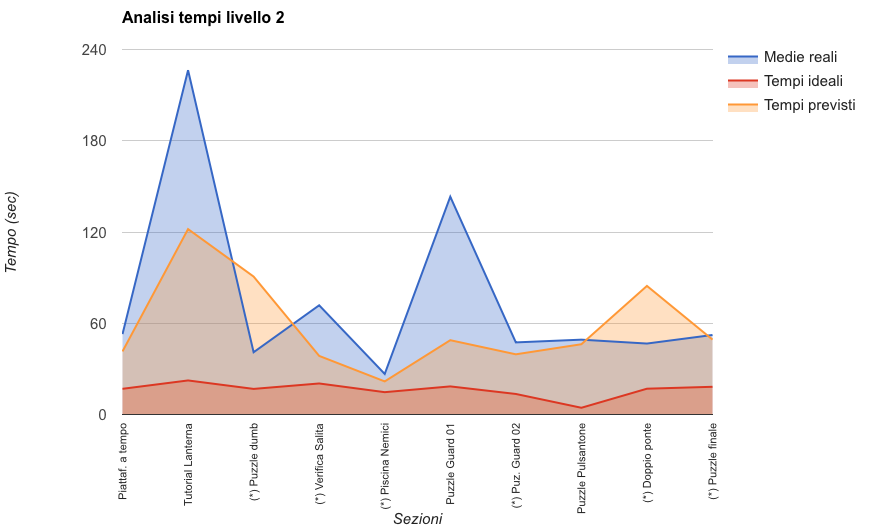
\includegraphics[scale=0.45]{images/risultati/test_01_analisi_tempi_02.png}}
\caption{Grafico analisi oggettiva dei tempi impiegati del livello 2.}
\label{fig:test_analisi_tempi_02}
\end{figure}

In due sezioni invece, ``Puzzle con dumb'' e ``Doppio ponte'' i tempi previsti sono risultati essere più bassi rispetto a quelli reali, questo è dovuto al fatto che i giocatori si sono spesso disinteressati del raccoglimento dei collezionabili di queste due sezioni, semplicemente proseguendo il livello.

Riguardo il terzo livello, è possibile vedere dalla  \myfig{\ref{fig:test_analisi_tempi_03}} che anche qui sono state solo 2 le sezioni i cui tempi previsti sono stati molto più bassi di quelli reali: ``Puzzle con bilancia'' e ``Mongolfiere''. Invece la sezione ``Puzzle porta'' ha avuto un tempo reale inferiore a quello ideale addirittura, sintomo del fatto che il rompicapo in questione è stato quasi totalmente ignorato dai giocatori.

\begin{figure}[h]
\centerline{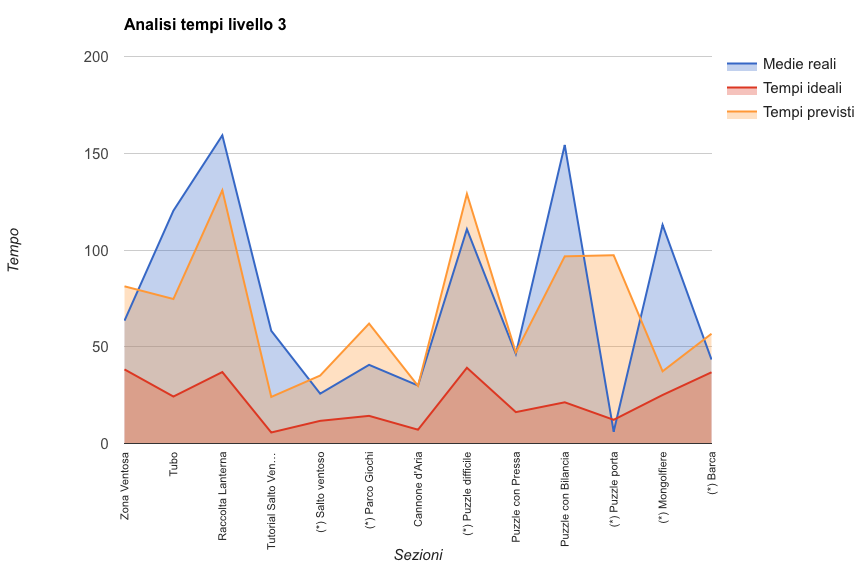
\includegraphics[scale=0.45]{images/risultati/test_01_analisi_tempi_03.png}}
\caption{Grafico analisi oggettiva dei tempi impiegati del livello 3.}
\label{fig:test_analisi_tempi_03}
\end{figure}

Altri dati al di sotto delle aspettative sono stati: i tempi di lettura dei contenuti informativi e le percentuali di raccoglimento dei collezionabili opzionali. 

La percentuale di ragazzi che si sono fermati a leggere i contenuti sbloccati è risultata essere bassa, ed i pochi ragazzi che hanno dedicato del tempo a questi contenuti, lo hanno fatto con un tipo in particolare di contenuto definito ``Fan Facts'', mentre l'altra tipologia, chiamata ``Oggetti'', è stata spesso ignorata. Vedremo un'analisi più approfondita di questi dati per il secondo test.

Per quanto riguarda i collezionabili raccolti, le percentuali di raccoglimento in generale è molto bassa, poco più dell'11\%. Questo fatto è dovuto probabilmente alla poca dimestichezza dei giocatori con la configurazione mouse e tastiera, in quanto, in buona parte dei casi, per prendere questi oggetti opzionali, è fondamentale avere un buon tempismo con i comandi di gioco. Vedremo un confronto sulle statistiche dei collezionabili fra il primo ed il secondo test durante l'analisi di quest'ultimo.

\newpage

%--------------
%--------------

\subsection{Revisione del design}
\label{revisione}
Considerati i feedback raccolti durante la prima sessione di testing, è stato ritenuto opportuno spendere del tempo per fare una revisione del design di alcune parti di gioco.
Buona parte del contenuto di questa revisione è già stato trattato nel Capitolo \ref{chap:game_design} sul game design, qui semplicemente vedremo di contestualizzare meglio il tutto.

Vediamo quindi i punti di revisione:

\begin{itemize}

\item Level Design: innanzitutto è stato modificato il level design di alcune sezioni di gioco, in particolare del primo livello, dove la curva di difficoltà era troppo ripida per essere il primo livello della demo. Sono state quindi tagliate alcune parti, il cui obiettivo originale era quello di rafforzare i tutorial di salto e coordinazione, fallendo nella maggior parte dei casi, e causando solo stress nel giocatore impreparato a tali ostacoli dopo solo qualche minuto di gioco.
\item NPC e quiz : si è scelto di includere degli NPC (Non Playable Character) al fine di catalizzare alcuni tutorial e la fruizione dei contenuti informativi, tramite, per esempio, alcuni quiz che premiano il giocatore con dei collezionabili opzionali.
\item Tutorial Lanterna: è stata rivista l'introduzione della Lanterna Magica, dando ad essa molta più enfasi, ed è stato rifatto anche il tutorial successivo che ne spiega l'uso.
\item Nuove meccaniche di gioco: sono state aggiunte al gioco nuove meccaniche di gioco tramite metafore di alcuni contenuti informativi, come per esempio le sezioni dedicate alle lenti e alla camera oscura, dove il giocatore è soggetto a delle regole che richiamino i meccanismi degli oggetti di interesse. Per esempio, nella sezione con le lenti, il giocatore può ingrandirsi o rimpicciolirsi, a seconda della lente attraverso cui passa.
\item Immagini contenuti Serious in game: si è pensato di attrarre l'attenzione del giocatore verso i contenuti informativi, mostrando questi in alcune sezioni di gioco tramite delle cornici giganti (come si vede in \myfig{\ref{fig:cornice_serious}}).
\item Supporto al controller: è stato supportato al 100\% l'uso del controller, così da agevolare quei giocatori meno abituati a mouse e tastiera.
\item Feedback contenuti sbloccati: poiché durante il primo test, le schede informative più lette sono risultate essere quelle della categoria ``Fun Facts'', si è pensato di uniformare il feedback visivo riguardo lo sblocco di tutti i contenuti, estendendo la grafica dei ``Fun Facts'' anche alle altre tipologie di schede informative.

\end{itemize}

\begin{figure}[h]
\centerline{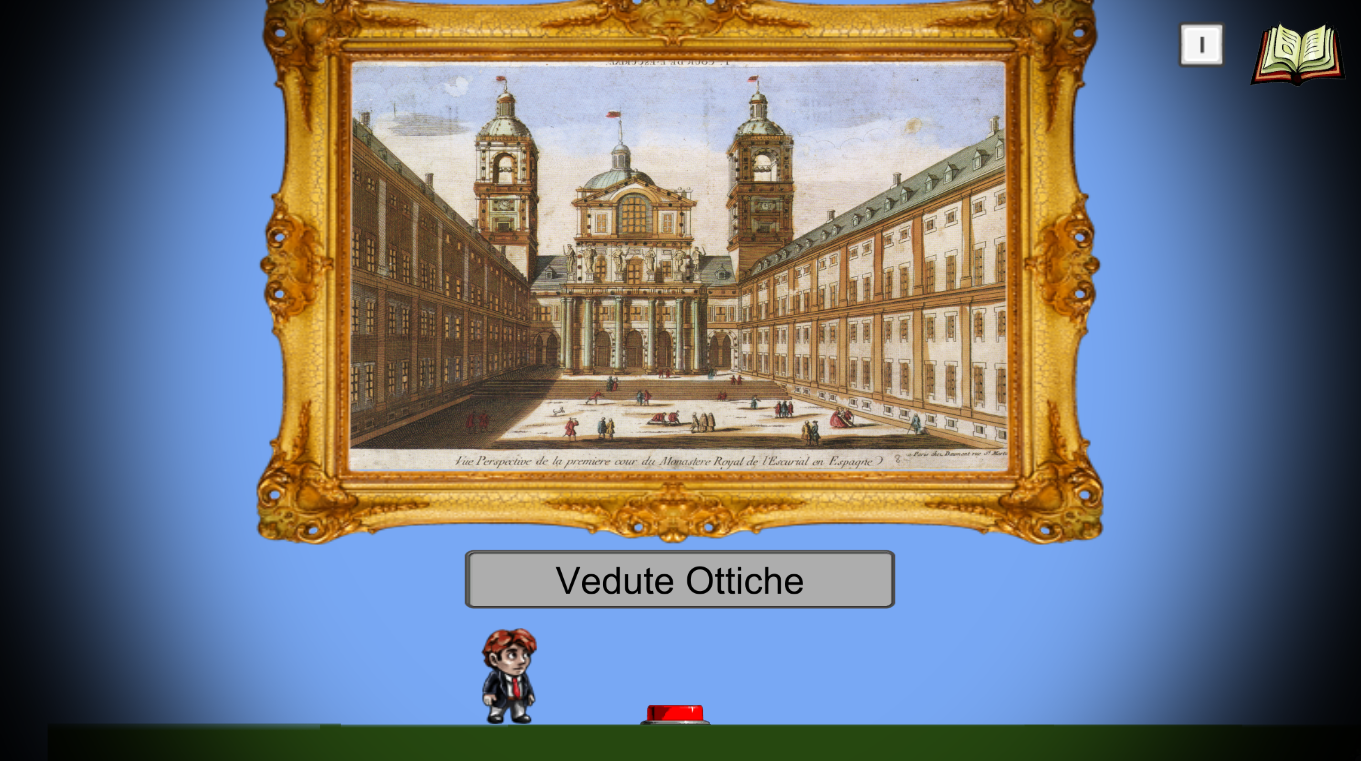
\includegraphics[scale=0.35]{images/risultati/cornice_serious.png}}
\caption{Cornice mostrante immagini dei contenuti informativi.}
\label{fig:cornice_serious}
\end{figure}

Nonostante il poco tempo a disposizione, circa 4 settimane, sono stati applicati i cambiamenti elencati. Si era ipotizzato di effettuare anche altri cambiamenti, ma le altre idee sono state accantonate e conservate per gli sviluppi futuri.

%--------------
%--------------

\subsection{Seconda sessione di testing}

%--------------

\subsubsection{Esito questionari}

I risultati del secondo round sono stati, in generale, più positivi rispetto a quelli del primo. Anche questa volta il gioco è stato recepito con grande coinvolgimento da parte dei tester.

\begin{figure}[h]
\centerline{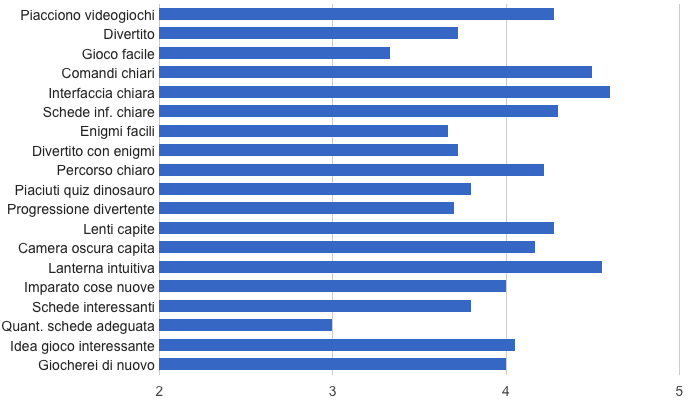
\includegraphics[scale=0.55]{images/risultati/test_02_questionario.png}}
\caption{Grafico sui questionari del secondo test.}
\label{fig:test-questionario02}
\end{figure}

Come già detto, i questionari consistevano in domande e affermazioni, sulle quali il giocatore doveva esprimere il suo indice di gradimento tramite la scala Likert.
Vediamo ora, in base ai risultati mostrati in \myfig{\ref{fig:test-questionario02}}, ciò che si è evinto dai questionari forniti (dei quali è mostrata una media delle risposte):

\begin{itemize}

\item Piacciono i videogiochi: con un voto medio superiore al 4, possiamo dire che il gioco è piaciuto abbastanza.
\item Divertito: il voto medio si aggira poco sotto del 4.
\item Facile: con un voto di 3,4 circa, il gioco è stato recepito con una difficoltà nella media.
\item Comandi chiari: la votazione media è stata superiore al 4, mostrando un miglioramento rispetto al primo test.
\item Interfaccia chiara: discorso simile al precedente, voto superiore al 4,5.
\item Schede inf. chiare: con una votazione superiore al 4 registriamo anche qui un miglioramento.
\item Enigmi facili: la votazione è risultata essere leggermente più alta rispetto al primo test, con un voto medio di poco inferiore al 4.
\item Percorso chiaro:  risultato molto simile alla prima sessione, con un voto di circa 4,2.
\item Piaciuti quiz dinosauro: i quiz sono stati graditi nella media, con un voto di circa 3,8.
\item Progressione divertente: voto medio poco al di sotto del 4.
\item Lenti capite: si è posta una domanda in particolare sulle lenti per capire quanto la meccanica attiva di gioco abbia avuto i suoi effetti sul giocatore, ed il risultato è stato abbastanza positivo visto il voto medio sopra il 4.
\item Camera oscura capita: stesso discorso delle lenti, l'argomento è stato recepito bene grazie anche all'esperienza attiva del giocatore. Voto poco sopra il 4.
\item Lanterna intuitiva: rispetto al primo test, il voto medio si è alzato parecchio, arrivando a 4,5, guadagnando quasi un punto.
\item Imparato nuove cose: si è registrato un miglioramento rispetto al primo test, passando da 3,4 a 4.
\item Schede interessanti: la risposta media è stata poco sopra il 3,8.
\item Idea gioco interessante: l'esito è stato positivo, assestandosi poco sopra il 4.
\item Giocherei di nuovo: anche qui, esito abbastanza positivo con valori intorno 4.

\end{itemize}

I fatti che possiamo dedurre da questa analisi riguardano in primo luogo i miglioramenti ai punti più critici del primo test. Come possiamo vedere tramite la \myfig{\ref{fig:test-confronto}}, cinque punti critici sono stati notevolmente migliorati.

\begin{figure}[h]
\centerline{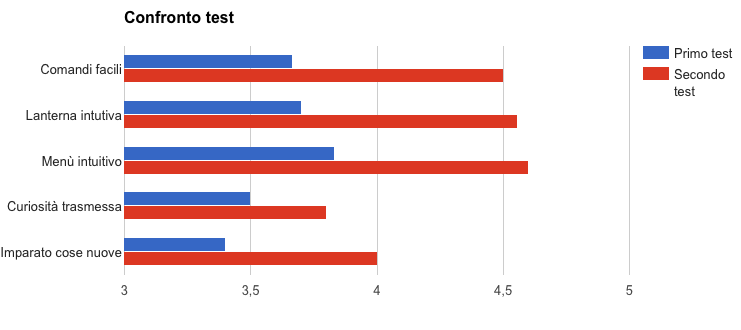
\includegraphics[scale=0.55]{images/risultati/test-confronto.png}}
\caption{Confronto dei risultati fra primo e secondo test.}
\label{fig:test-confronto}
\end{figure}

\subsubsection{Esito analisi oggettive}

Il miglioramento della giocabilità della demo è stato confermato anche dalla lettura delle analisi oggettive, difatti, facendo un confronto fra i grafici del livello uno di primo e secondo test (vedi \myfig{\ref{fig:test-confronto-tempi1}}) possiamo notare che nel grafico del secondo test, l'andamento dei tempi reali segue abbastanza bene quello dei tempi previsti, cosa non sempre vera nel grafico del primo test, dove sono presenti dei picchi della funzione blu (tempi reali) che si discostano parecchio dai relativi punti della funzione arancione (tempi previsti).

\begin{figure}[h]
\centerline{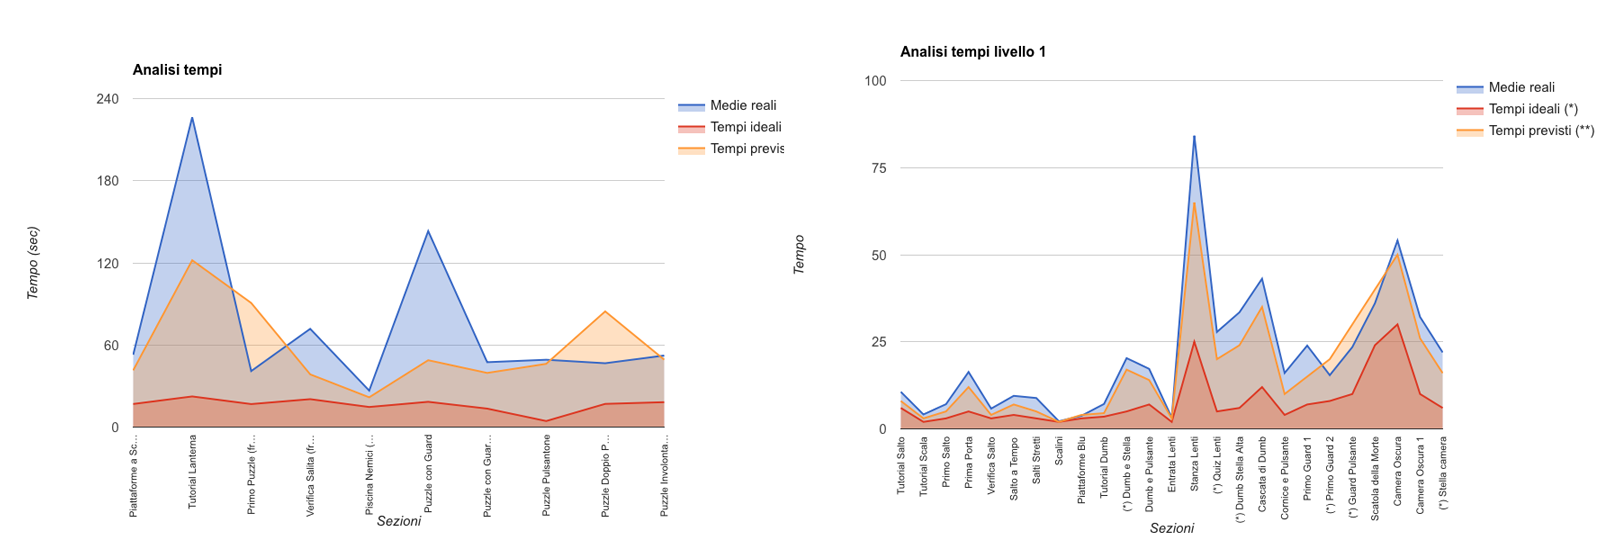
\includegraphics[scale=0.3]{images/risultati/test-confronto-tempi1.png}}
\caption{Confronto dei risultati fra primo e secondo test del livello 1.}
\label{fig:test-confronto-tempi1}
\end{figure}

Il miglioramento è presente anche per il secondo e terzo livello, come è possibile notare dalla \myfig{\ref{fig:test-confronto-tempi2-3}} (sulla sinistra sono presenti i grafici del primo test, mentre sulla destra quelli del secondo).

\begin{figure}[h]
\centerline{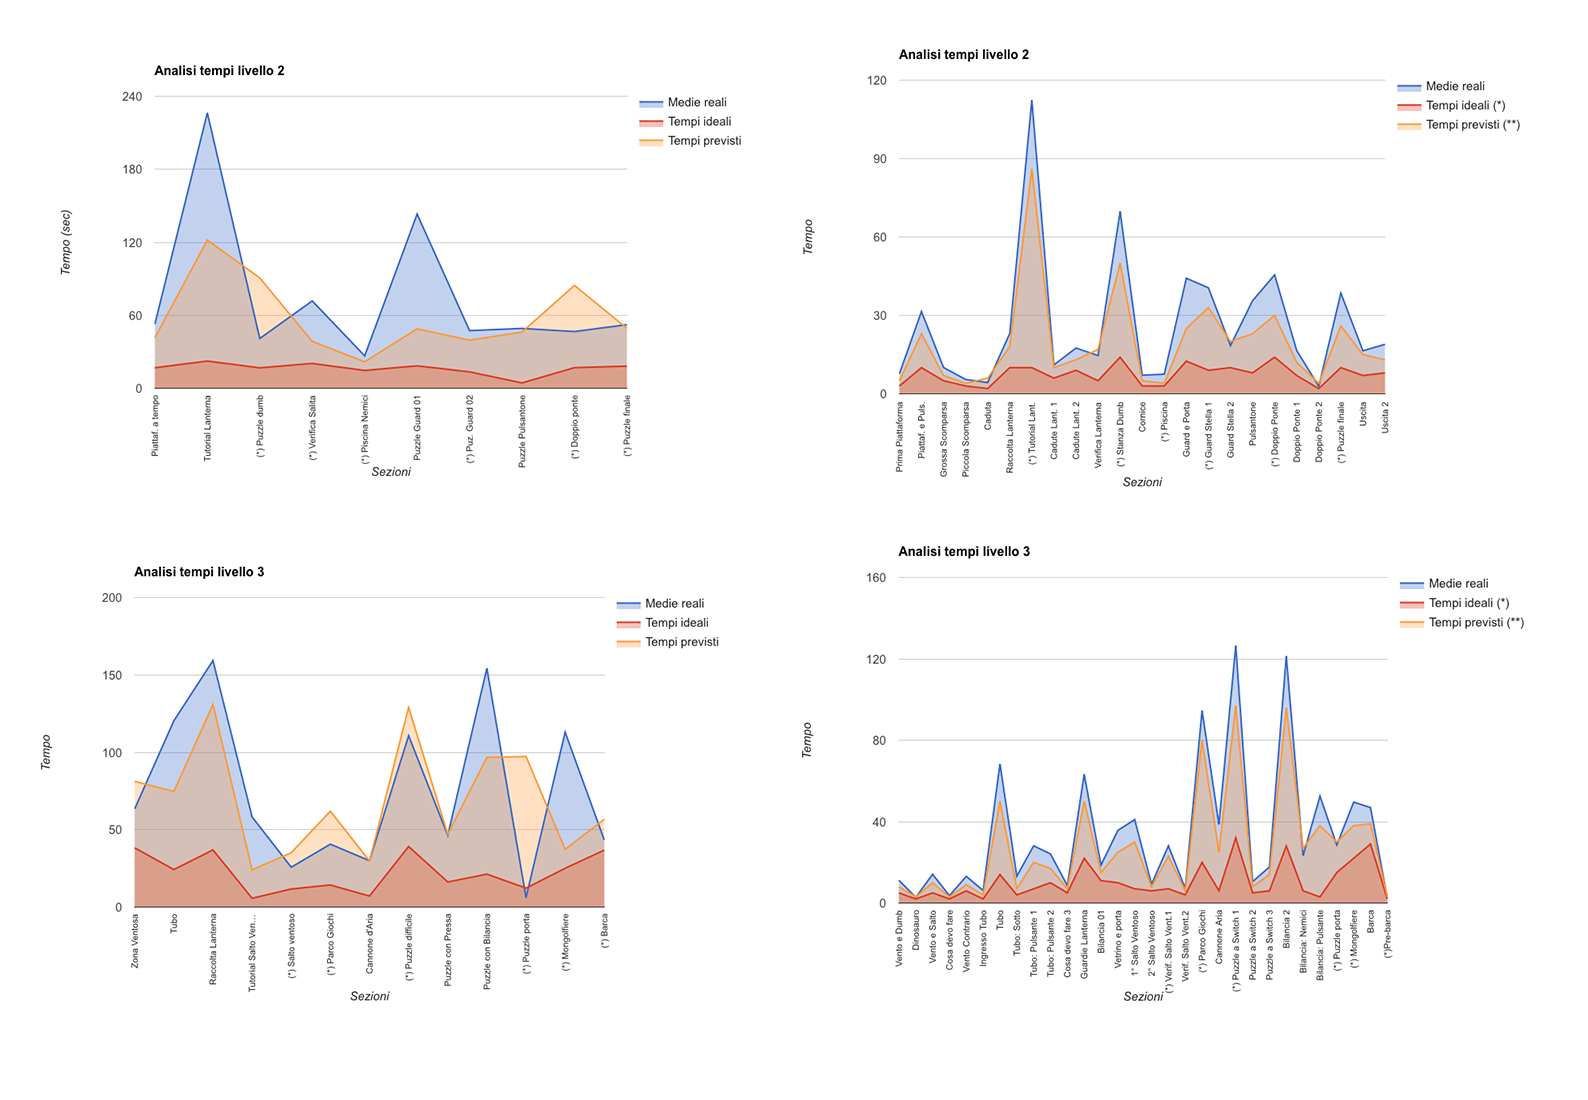
\includegraphics[scale=0.3]{images/risultati/test-confronto-tempi2-3.png}}
\caption{Confronto dei risultati fra primo e secondo test dei livelli 2 e 3.}
\label{fig:test-confronto-tempi2-3}
\end{figure}

Per quanto riguarda l'analisi dei dati sulla fruizione dei contenuti informativi, durante il primo test la percentuale di persone interessate alle varie schede è stata mediamente del 6\% riguardo gli oggetti, e del 30\% riguardo i ``Fun Facts'', quindi statistiche davvero molto basse. Questa volta invece sono stati registrati dei dati molto interessanti e positivi.

Vediamo per esempio le percentuali di giocatori interessanti alle varie schede informative, e i tempi medi di lettura dedicati (vedi \myfig{\ref{fig:test-percTempiSchede}}).

\begin{figure}[h]
\centerline{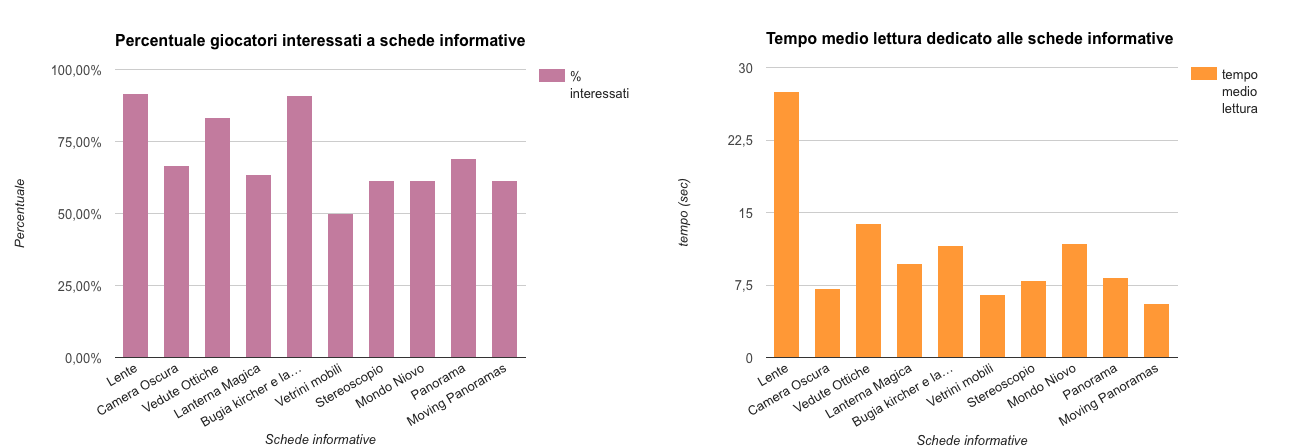
\includegraphics[scale=0.35]{images/risultati/test_seriousStats.png}}
\caption{Grafici riguardo le percentuali dei giocatori che hanno letto che schede informative, e il tempo medio dedicato per scheda.}
\label{fig:test-percTempiSchede}
\end{figure}

Nota bene: è stata fatta una scelta arbitraria per definire quale fosse un giocatore minimamente interessato ad un contenuto informativo, questo per essere etichettato come tale deve aver dedicato almeno 2 secondi al contenuto.

Possiamo notare che le percentuali sono tutte piuttosto alte, con picchi delle schede ``Lenti'' e ``Lanterna sbagliata''. La scheda sulle lenti è la prima del gioco, il fatto che quasi tutti l'abbiano aperta è un buon segno che conferma la chiarezza dell'interfaccia di gioco riguardo lo sblocco e la lettura delle schede informative. Le conclusioni possibili riguardo queste analisi sono quasi tutte arbitrarie, in quanto non è possibile avere completa certezza sul fatto che i giocatori durante il tempo per il quale hanno avuto la scheda informativa aperta, la stavano davvero leggendo.

Difatti, per capire se un giocatore abbia appreso o meno qualcosa riguardo il pre-cinema, si è tentato di farlo tramite l'aggiunta di appositi quiz, uno per livello, nei quali si ponevano al giocatore semplici domande, a risposta multipla. Giudicando come preparati i giocatori che hanno indovinato la risposta al primo colpo, le statistiche estratte dai dati sono visibili in \myfig{\ref{fig:test-quiz}}.

\begin{figure}[h]
\centerline{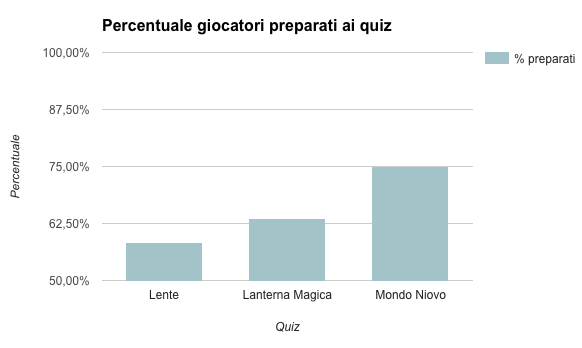
\includegraphics[scale=0.65]{images/risultati/test-quiz.png}}
\caption{Grafico della percentuale dei giocatori preparati ai quiz.}
\label{fig:test-quiz}
\end{figure}

Anche queste statistiche non possono essere precise al 100\%, in quanto, un giocatore potrebbe aver scelto a caso la risposta ed indovinato al primo colpo.

Un fatto degno di nota di questa analisi, è la percentuale di interessamento alla scheda informativa della Lanterna Magica, per la quale, ``solo'' il 63\% dei tester si è interessato, nonostante siano le informazioni potenzialmente più esplicative del gioco. Questo fatto può essere dovuto alla posizione non proprio comoda dove si sblocca il contenuto. In questo punto del gioco, il player ha appena superato il tutorial della Lanterna, e sta per usare nuovamente questa per superare una sezione puzzle-platform. Probabilmente, a questo punto, l'attenzione del player è rivolta totalmente verso la parte di livello da superare, al punto da ignorare la scheda appena sbloccata.

Un altro dato interessante riguarda le modalità di lettura delle schede informative, cioè il momento in cui il giocatore accede alle informazioni sbloccate. Nonostante sia possibile accedere ai contenuti sbloccati anche in un secondo momento, la maggior parte dei tester che ha aperto le schede informative, l'ha fatto nel momento in cui queste venivano sbloccate, e non in un secondo momento. Le schede che non sono state aperte subito, in genere non sono state aperte neanche dopo.

Vediamo, infine, l'analisi sulla raccolta dei collezionabili opzionali, confrontando i risultati del primo test con quelli del secondo.

Nota bene: alcune stelle sono state riposizionate prima del secondo test, soprattutto nel primo livello, un po meno nel secondo, mentre il terzo è rimasto invariato.

Le percentuali di raccoglimento del secondo test sono nettamente superiori, risultato in buona parte da attribuire ad un flow di gioco più lineare e ai feedback aggiunti ove mancavano nel primo test. Ha influito su questi dati anche l'uso di device ad hoc per l'utente inesperto dell'uso di mouse e tastiera, ciò ha permesso agli utenti di avere maggiore coordinazione e precisione ove necessario. Un'altra possibile motivazione dell'alto numero di collezionabili presi, può essere il fatto che il giocatore medio del secondo test aveva un'età (16 anni) superiore al giocatore del primo test (12-14 anni), presentando una dimestichezza ed esperienza di gioco in media superiori.

\begin{figure}[h]
\centerline{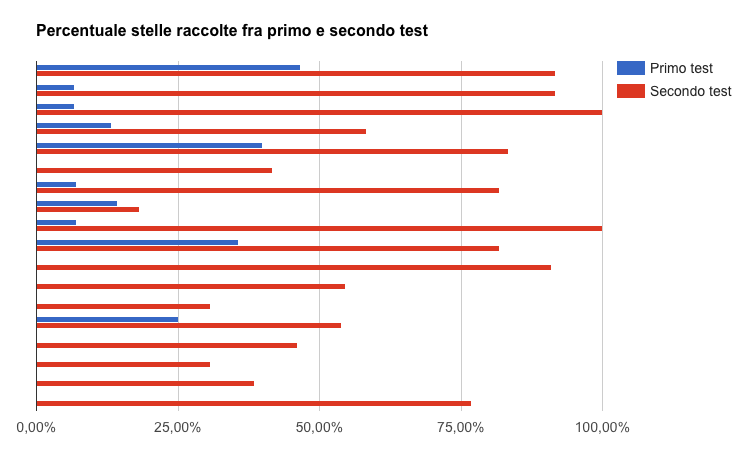
\includegraphics[scale=0.6]{images/risultati/test-stelle.png}}
\caption{Grafico della percentuale dei giocatori che hanno raccolto le stelle, durante primo e secondo test.}
\label{fig:test-stelle}
\end{figure}

\newpage